\documentclass[12pt,a4paper]{article}
\usepackage{graphicx, color}
\usepackage[margin=2cm]{geometry}
\usepackage{multirow}
\usepackage{sectsty}
\usepackage{amssymb}
\usepackage{wrapfig}
\usepackage{natbib}
\usepackage{hyperref}
%\usepackage{url}
%\usepackage[pdftex]{graphicx}

\sectionfont{
%	\sectionrule{0pt}{0pt}{-5pt}{1pt}
}
\begin{document}
\title{\color{red} The Lazy Man's Cycle Starter}
\maketitle

\begin{table}[ph]
\large
\centering
\begin{tabular}{c c c}
\hline
GroupName &RollNumber &Name\\
\hline 
\multirow{3}{*}{!JustCoders} &140050031 &C Vishwesh\\ &140070003 &Saurabh Garg\\&140070031 &Aviral Kumar\\
\hline
\end{tabular}
\end{table}
\pagebreak
\section{Motivation} \label{mot}

While surfing through some science stuff on the Internet we came across a very new idea of riding a cycle having square wheels on a road made of Catenary curves (\ref{eqn})
(\textit{https://www.sciencenews.org/ article/riding-square-wheels}). This seemed quite interesting to us. We had earlier never heard of or thought about such an idea, and therefore we decided to make a Rube Goldberg Machine to make such a bicycle without any paddles move on such a road. 
\section{Introduction} \label{intro}
%\floatstyle{boxed}

\begin{figure}[ht!]
\centering
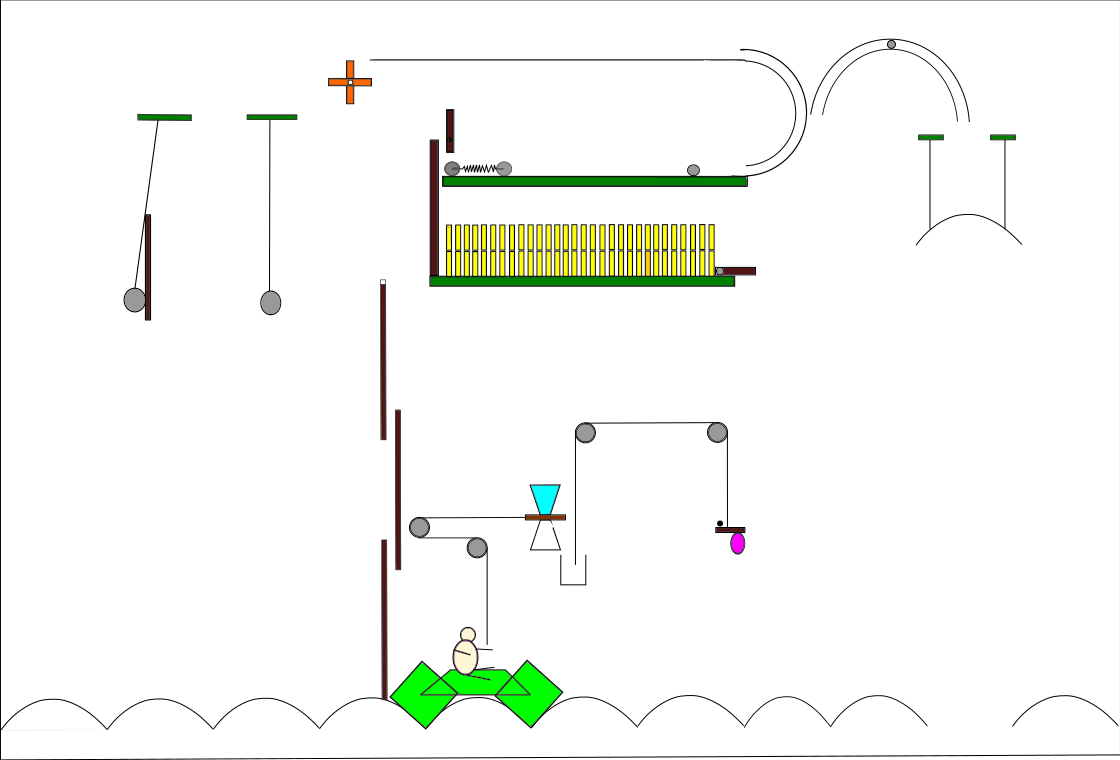
\includegraphics[scale=0.45]{mbox2d.png}
\caption{Preliminary Design \label{img}}
\end{figure} 
%\restylefloat{figure}
%\end{figure}
As decribed in section \ref{mot}, we are planning to make a \textit{Cycle Starter Rube Goldberg Machine} as our project. There's a lazy man who doesn't want to paddle his cycle down the road with a hole in between. When he pulls down a rope hanging just in front oh him, a chain of events is triggered which eventually gives the man a forward impulse to move to the front. Secondly, this also completes the path by filling the hole in the road and thus makes the life of the lazy man easier.\\ \\

%There is a man who is stuck on his cycle having square shaped wheels on a road which is made of Catenary curves\textsuperscript{1}. In order to move, he pulls a string which is connected through two pulleys to a plank which partitions a body similar in shape to an hourglass which has water in its upper half and a hole in its lower half.When this plank gets pulled, the water falls down which brings a balloon into motion which inturn hits the plank above. This collision causes a wave of domino collisions which then leads to movement of a 2 ball system connected by a string. 

%\end 
\section{Description} \label{desp}
\subsection{Working Principle} \label{work}
\begin{list}{$\cdot$}{\leftmargin=3.5em}
\item Firstly, make a road which is made of multiple Catenary curves \ref{eqn} \ref{road} but with a hole in place of one of the curves
\item A man is sitting on his bicycle having square wheels on the road. He is so lazy, that he doesn't want to paddle his bicycle. So he pulls a string hanging in front of him which triggers a chain of events.
\item At first, this jerk removes the plank partitioning the hour glass \ref{hg}. It's upper half is filled with water and the lower half has a hole. The water flows down and rushes out of the hole into the beaker, Thus making the system of the beaker unstable. The motion of this system turns the right side plank thus freeing the balloon which moves up.
\item The balloon hits the plank above which collides with the double layered dominos stack \ref{dom}. Thus energy is transferred to the dominos.
\item Dominos inturn transfer energy to the pivoted rod at the end of the plank, which transfers energy to the spring-ball \ref{spring} \ref{hooke} system, bring it into motion.
\item This sets up a ball into motion which moves up the circular track and hits a fan kept near its end which deviates it and gives it a sufficient velocity that it is able to hit the plank stopping the pendulum from moving.
\item This stopper plank breaks and the pendulums collide, therby starting a chain of collisions between the planks and finally imparting a linear impulse to the square wheel.
\item Meanwhile, the balloon moves up into the semi-circular tube and displaces the ball which falls over the piece of the road hanging above and breaks the strings holding it. The piece moves down and completes the road.
\end{list}

\subsection{What and when are we gonna do?} \label{what}
\begin{list}{$\cdot$}{\leftmargin=3.5em}
\item We'll design the floor, cycle and the man first using catenary curves.
\item Then we'll design the hourglass, pulley systems, rods and the balloon.
\item Post doing this, we shall design the domino chain and the spring mass system.
\item Finally, We shall join these with appropriate joints and connections as mentioned in the image \ref{img} and integrate them all together.    
\end{list}

\subsection{Task Distribution}{\leftmargin=3.5em} \label{time}
\begin{list}{$\cdot$}{\leftmargin=3.5em}
\item As this is a team task, we all plan to sit together while doing any work related to the project. The exact distribution of work has not been decided until yet and will depend on our pace of doing work.
\end{list}
\pagebreak
\section{Physics Behind the Project} \label{phy}
\subsection{Equations involved}
\begin{list}{$\cdot$}{\leftmargin=3.5em}
\item Newton's Second Law $$\vec{F}=M\vec{a}$$ \label{second}
\item  \label{uni} $2^{nd}$ Equation of Motion with Uniform Acceleration $$\vec{S}= \vec{u}t + \frac{1}{2}\vec{a}t^2$$ 
\item Conservation of Momentum $$\sum\vec{p_i}=\sum\vec{p_f}$$ \label{mom}
\item Newton's Law of Rotational Motion $$\sum\vec{\tau_{ext}}=I\vec{\alpha}$$\label{rot}
\item Time Period of a Pendulum $$T=2\pi{\sqrt\frac{l}{g}}$$ \label{tp}
\item \label{eqn} Equation of a Catenary Curve $$y=a cosh{(\frac{x}{a})}$$ 
\item Hooke's Law $$\vec{F}=-k\vec{x}$$ \label{hooke}
\end{list}

\pagebreak
\section{Internal Components} \label{ic}
Some of the innovations in the project are: \\ 
\subsection{A cycle with square wheels} \label{sqr}
\begin{wrapfigure}[4]{l}{0.40\textwidth}
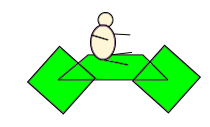
\includegraphics[width=0.75\linewidth]{cycle.png}
\caption {A cycle with square wheels}
\label{wrapfig}
\end{wrapfigure}
A cycle has circular wheels. The entire idea of making a cycle with square wheels seems quite interesting and therefore we chose to make it.
\\[10ex]
\subsection{Road made of Catenary curves} \label{road}
\begin{wrapfigure}[4]{l}{0.50\textwidth}
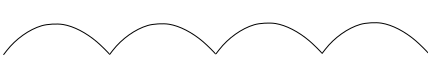
\includegraphics[width=0.8\linewidth]{road.png}
\caption{Some pieces of Catenary curves}
\end{wrapfigure}
A road which can facilitate easy motion of the cycle with square wheels. The shape of the road is not arbitrary, it is a special kind of a curve called \textit{Catenary Curve} \ref{eqn}.
\\[3ex]
\subsection{Hourglass} \label{hg}
\begin{wrapfigure}[6]{l}{0.50\textwidth}
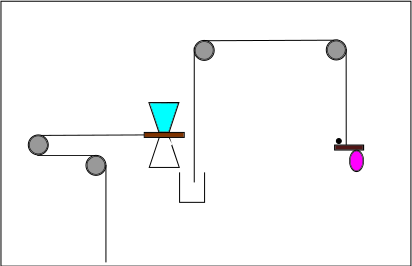
\includegraphics[width=0.8\linewidth]{hg.png}
\caption{Hourglass filled half with water}
\end{wrapfigure}
This is the system of pulleys consisting of an hourglass whose upper half is filled with water and is partitioned into two halves by a plank. Moreover there is a balloon, stuck below a plank which stays in its position due to a stopper (peg) above it.
\\[10ex]
\subsection{Dominos} \label{dom}
\begin{wrapfigure}[4]{l}{0.50\textwidth}
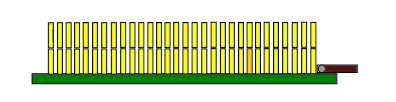
\includegraphics[width=0.8\linewidth]{domnios.png}
\caption{A double layered stack}
\end{wrapfigure}
Dominos cause a transfer of energy from one side to the other on the plank. Also they would give a nice look to the viewer watching the simulation. 
\\[20ex]
\subsection{Spring Mass System} \label{spring}
\begin{wrapfigure}[4]{l}{0.40\textwidth}
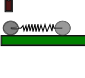
\includegraphics[width=0.4\linewidth]{spring.png}
\caption{Spring-Mass System}
\end{wrapfigure}
Two bodies are connected by a spring and kept on top of a plank. This spring-mass problem is a nice problem in mechanics of moentum conservation and it would be nice to use such an oscillatory system in the machine.  
\\[20ex]
\section{Conclusions} \label{conc}
In this version of the Rube Goldberg Machine, we have tried to implement a complex mechanism to do a simple task i.e. starting a cycle which forms the essential basis of the Rube Goldberg Machine. We will implement everything mentioned here and would try to add more features to the project. 

\bibliographystyle{unsrt}%Used BibTeX style is unsrt
\bibliography{refer}
\cite{ref1} 
\cite{ref2}
%\label{bib}
%\begin{thebibliography}{9}
%\bibitem{first}
%Square wheeled cycle in reality: \textit{\href{https://www.sciencenews.org/article/riding-square-wheels}{https://www.sciencenews.org/article/riding-square-wheels}}
%\bibitem{second}
%Square Wheeled Cycle driven on a Catenary road:\textit{\href{https://www.youtube.com/watch?v=0BtZcmEkFsI}{https://www.youtube.com/watch?v=0BtZcmEkFsI}}
%\bibitem{third}
%Mathematical equations of Catenary curve: \textit{\href{http://mathworld.wolfram.com/Catenary.html}{http://mathworld.wolfram.com/Catenary.html}}
%\end{thebibliography}
\end{document}

